\section{Supplementary results}
\label{app:supplementary-results}

\subsection{Additional two-dimensional comparisons}
\label{app:additional-2d-comparisons}

The correlated shape difference spans both small- and moderate-variance
directions of the published covariance. For a retained eigenpair
$(\lambda_k,u_k)$, the contribution to the distance in
Sec.~\ref{sec:muon-cross-section-comparison} is
$(u_k^{\mathsf T}\Delta)^2/\lambda_k$. The ten smallest-eigenvalue modes
carry $9.6\%$ of the distance. Among the six largest contributors, three
are concentrated in the highest-$p_\parallel$ bins and have
$\lambda_k/\lambda_{\max}\lesssim4\times10^{-9}$, while the other three lie
at lower $p_\parallel$ and have relative eigenvalues between
$4\times10^{-6}$ and $6\times10^{-5}$
(Figs.~\ref{fig:tension} and~\ref{fig:tensionmodes}).
Figures~\ref{fig:ptslices} and~\ref{fig:pzslices} show
the cross sections in the original muon bins.

\begin{figure}[H]
  \centering
  \includegraphics[width=0.49\textwidth]{tension_spectrum}\hfill
  \includegraphics[width=0.49\textwidth]{tension_chi2_map}
  \caption{Many modes contribute to the descriptive $\chi^2$, and the bin contributions
  can have either sign because the covariance is correlated. The panels show
  the published-covariance spectrum, the cumulative $\chi^2$ ranked by mode
  contribution, and the signed bin contributions
  $\Delta_i(V_{\mathrm{pub}}^+\Delta)_i$. The shared-data comparison is descriptive.}
  \label{fig:tension}
\end{figure}


\begin{figure}[H]
  \centering
  \includegraphics[width=\textwidth]{tension_mode_maps}
  \caption{Three of the six published-covariance eigenvectors with the largest
  contributions to the descriptive $\chi^2$, in panels (a), (b), and (d),
  concentrate at the highest $p_\parallel$. The panels are in decreasing order
  of contribution. The colors show eigenvector components, whose overall signs
  are arbitrary.}
  \label{fig:tensionmodes}
\end{figure}

\begin{figure}[H]
  \centering
  \includegraphics[width=\textwidth]{MEFHC_5iter_xsec_paper_pt_slices}
  \caption{In all 14 $p_T$ slices, the OmniFold points move toward the published values
  relative to the Tune~v1 prior. The panels show rescaled double-differential
  cross sections versus $p_\parallel$. OmniFold bars show event-weight
  statistics only, and the panel $\chi^2/n$ compares OmniFold with the prior.}
  \label{fig:ptslices}
\end{figure}

\begin{figure}[H]
  \centering
  \includegraphics[width=\textwidth]{MEFHC_5iter_xsec_paper_pz_slices}
  \caption{In all 16 $p_\parallel$ slices, the unfolding draws the central values toward
  the published points. The panels show rescaled double-differential cross
  sections versus $p_T$. Bars and panel distances follow Fig.~\ref{fig:ptslices}.}
  \label{fig:pzslices}
\end{figure}

The distance to the publication depends on the learner and the background
subtraction. At fixed LightGBM settings and training seed, refined
negative-weight subtraction reduces $\chi^2$ per bin from \chiPaperPurity{} to \chiPaper{}.
With purity subtraction, the distance is 2.64--2.75 across ten LightGBM
seeds, $2.70\pm0.04$ for the histogram-based implementation in
\textsc{scikit-learn}, and \chiPaperExact{} for exact-split gradient boosting.

Binned IBU gives a distance to the publication of \fvval{c2c1-dibu-mid-lo}--\fvval{c2c1-dibu-mid-hi} per bin
for two to fifteen iterations, \fvval{c2c1-dibu-k20} at twenty iterations, and \fvval{c2c1-dibu-k1} at one.
At fixed IBU settings, replacing the classifier-refined reconstructed
target with the binwise data-minus-background histogram changes the
OmniFold--IBU distance per bin from \fvval{ibusd-k5-ref} to \fvval{ibusd-k5-sig} at five iterations
and from \fvval{ibusd-k10-ref} to \fvval{ibusd-k10-sig} at ten. These distances use the published
covariance as a common descriptive metric for results that share data.

\subsection{Higher-dimensional projections and generator comparisons}
\label{app:higher-dimensional-projections}
\label{sec:fived16-gen-target}
\label{sec:eavailw-band}
\label{sec:3d-models}

The reconstructed controls reproduce the simulated pairwise correlations
to within 0.02 for all ten pairs (Fig.~\ref{fig:control-corner}). The two
largest Pearson coefficients in data are 0.82 for $(E_{\mathrm{avail}},q_3)$
and 0.74 for $(E_{\mathrm{avail}},W)$. In simulated signal, migration
in the muon momenta occurs mainly to the same or neighboring bins.
Migration is broader for the observables that use calorimetry. The median
same-bin probability across truth bins ranges from 0.58 to 0.61 on
each of the five axes.

\begin{figure}[H]
  \centering
  \includegraphics[width=\textwidth]{control_corner}
  \caption{The Pearson coefficients in data and simulation agree closely over the
  displayed range, which omits the wide catch bins. Below the diagonal are the
  reconstructed pair densities for exposure-scaled simulated signal plus
  background, and on the diagonal the data and simulation marginals.}
  \label{fig:control-corner}
\end{figure}

The predictions differ most visibly in available energy in the 3D
projections (Fig.~\ref{fig:3dmodels}). The plotted GENIE and NuWro
predictions in both comparisons use the flux correction described in
Appendix~\ref{app:choices-after-results}. In the \resFiveAxis{}, all four predictions in Fig.~\ref{fig:eavailWband} fall below the central value
in the corner $E_{\mathrm{avail}}\geq0.8~\mathrm{GeV}$ and
$W\geq1.8~\mathrm{GeV}$. The data-to-prediction ratios there are \genRatioCornerLo{} for
both GENIE configurations, \genRatioCornerHi{} for NuWro, and \gibuuCorner{} for GiBUU, whose sample
ends at $E_\nu=\fvval{cmodel-gibuu-enu}~\mathrm{GeV}$.

\begin{figure}[H]
  \centering
  \includegraphics[width=\textwidth]{generators_vs_unfolded_band_central}
  \caption{The generator predictions follow the muon-momentum shapes of the refined 3D
  central values more closely than the available-energy shape. The panels show
  single-variable projections against GENIE, MINERvA Tune~v1, NuWro, and
  GiBUU. The 3D result has no reported covariance.}
  \label{fig:3dmodels}
\end{figure}

\begin{figure}[H]
  \centering
  \includegraphics[width=\textwidth]{eavailW_band}
  \caption{Both GENIE predictions are $\genieWmidLo{}\%$--$\genieWmidHi{}\%$ above the
  unfolded central value at $1.4\leq W<1.8~\mathrm{GeV}$. The panels show the
  $E_{\mathrm{avail}}$ (left) and $W$ (right) marginals of the \resFiveAxis{}
  and four generator predictions, and below them each prediction divided by the
  unfolded central value. The comparison uses central values only.}
  \label{fig:eavailWband}
\end{figure}

The sixteen-cell uncertainties vary substantially in composition across
the reporting regions. Tables~\ref{tab:sixteen-cell-uncertainty-groups}
and~\ref{tab:sixteen-cell-uncertainty-response} give the diagonal contributions to Eq.~\eqref{eq:sixteen-cell-covariance}.
The correlations in Table~\ref{tab:sixteen-cell-correlations} and the
total standard deviations in Table~\ref{tab:sixteen-cell-cross-sections}
specify the reported covariance to the printed precision.

\begin{table}[tbp]
  \centering
  \caption{Per-cell relative standard deviations in percent from the
  statistical, systematic, and prior-shape terms. The statistical, flux,
  interaction, detector, lateral, and normalization covariances sum to
  $C_e$. The training-seed contribution is zero. The cell definitions are
  in Table~\ref{tab:five-dimensional-regions}.}
  \label{tab:sixteen-cell-uncertainty-groups}
  \label{tab:fived16-groups}
  \small
  \begin{tabular}{@{}l*{9}{r}@{}}
    \toprule
    Cell & Stat. & Flux & Int. & Det. & Lat. & Norm. & $C_e$ & $C_{\mathrm{model}}$ & $C_{\mathrm{total}}$ \\
    \midrule
    R00 & \fvval{sig-stat-R00} & \fvval{sig-flux-R00} & \fvval{sig-interaction-R00} & \fvval{sig-detector-R00} & \fvval{sig-lateral-R00} & \fvval{sig-normalization-R00} & \fvval{sig-C_e-R00} & \fvval{sig-C_model-R00} & \fvval{sig-C_total-R00} \\
    R01 & \fvval{sig-stat-R01} & \fvval{sig-flux-R01} & \fvval{sig-interaction-R01} & \fvval{sig-detector-R01} & \fvval{sig-lateral-R01} & \fvval{sig-normalization-R01} & \fvval{sig-C_e-R01} & \fvval{sig-C_model-R01} & \fvval{sig-C_total-R01} \\
    R02 & \fvval{sig-stat-R02} & \fvval{sig-flux-R02} & \fvval{sig-interaction-R02} & \fvval{sig-detector-R02} & \fvval{sig-lateral-R02} & \fvval{sig-normalization-R02} & \fvval{sig-C_e-R02} & \fvval{sig-C_model-R02} & \fvval{sig-C_total-R02} \\
    R03 & \fvval{sig-stat-R03} & \fvval{sig-flux-R03} & \fvval{sig-interaction-R03} & \fvval{sig-detector-R03} & \fvval{sig-lateral-R03} & \fvval{sig-normalization-R03} & \fvval{sig-C_e-R03} & \fvval{sig-C_model-R03} & \fvval{sig-C_total-R03} \\
    \addlinespace[2pt]
    R04 & \fvval{sig-stat-R04} & \fvval{sig-flux-R04} & \fvval{sig-interaction-R04} & \fvval{sig-detector-R04} & \fvval{sig-lateral-R04} & \fvval{sig-normalization-R04} & \fvval{sig-C_e-R04} & \fvval{sig-C_model-R04} & \fvval{sig-C_total-R04} \\
    R05 & \fvval{sig-stat-R05} & \fvval{sig-flux-R05} & \fvval{sig-interaction-R05} & \fvval{sig-detector-R05} & \fvval{sig-lateral-R05} & \fvval{sig-normalization-R05} & \fvval{sig-C_e-R05} & \fvval{sig-C_model-R05} & \fvval{sig-C_total-R05} \\
    R06 & \fvval{sig-stat-R06} & \fvval{sig-flux-R06} & \fvval{sig-interaction-R06} & \fvval{sig-detector-R06} & \fvval{sig-lateral-R06} & \fvval{sig-normalization-R06} & \fvval{sig-C_e-R06} & \fvval{sig-C_model-R06} & \fvval{sig-C_total-R06} \\
    R07 & \fvval{sig-stat-R07} & \fvval{sig-flux-R07} & \fvval{sig-interaction-R07} & \fvval{sig-detector-R07} & \fvval{sig-lateral-R07} & \fvval{sig-normalization-R07} & \fvval{sig-C_e-R07} & \fvval{sig-C_model-R07} & \fvval{sig-C_total-R07} \\
    \addlinespace[2pt]
    R08 & \fvval{sig-stat-R08} & \fvval{sig-flux-R08} & \fvval{sig-interaction-R08} & \fvval{sig-detector-R08} & \fvval{sig-lateral-R08} & \fvval{sig-normalization-R08} & \fvval{sig-C_e-R08} & \fvval{sig-C_model-R08} & \fvval{sig-C_total-R08} \\
    R09 & \fvval{sig-stat-R09} & \fvval{sig-flux-R09} & \fvval{sig-interaction-R09} & \fvval{sig-detector-R09} & \fvval{sig-lateral-R09} & \fvval{sig-normalization-R09} & \fvval{sig-C_e-R09} & \fvval{sig-C_model-R09} & \fvval{sig-C_total-R09} \\
    R10 & \fvval{sig-stat-R10} & \fvval{sig-flux-R10} & \fvval{sig-interaction-R10} & \fvval{sig-detector-R10} & \fvval{sig-lateral-R10} & \fvval{sig-normalization-R10} & \fvval{sig-C_e-R10} & \fvval{sig-C_model-R10} & \fvval{sig-C_total-R10} \\
    R11 & \fvval{sig-stat-R11} & \fvval{sig-flux-R11} & \fvval{sig-interaction-R11} & \fvval{sig-detector-R11} & \fvval{sig-lateral-R11} & \fvval{sig-normalization-R11} & \fvval{sig-C_e-R11} & \fvval{sig-C_model-R11} & \fvval{sig-C_total-R11} \\
    \addlinespace[2pt]
    R12 & \fvval{sig-stat-R12} & \fvval{sig-flux-R12} & \fvval{sig-interaction-R12} & \fvval{sig-detector-R12} & \fvval{sig-lateral-R12} & \fvval{sig-normalization-R12} & \fvval{sig-C_e-R12} & \fvval{sig-C_model-R12} & \fvval{sig-C_total-R12} \\
    R13 & \fvval{sig-stat-R13} & \fvval{sig-flux-R13} & \fvval{sig-interaction-R13} & \fvval{sig-detector-R13} & \fvval{sig-lateral-R13} & \fvval{sig-normalization-R13} & \fvval{sig-C_e-R13} & \fvval{sig-C_model-R13} & \fvval{sig-C_total-R13} \\
    R14 & \fvval{sig-stat-R14} & \fvval{sig-flux-R14} & \fvval{sig-interaction-R14} & \fvval{sig-detector-R14} & \fvval{sig-lateral-R14} & \fvval{sig-normalization-R14} & \fvval{sig-C_e-R14} & \fvval{sig-C_model-R14} & \fvval{sig-C_total-R14} \\
    R15 & \fvval{sig-stat-R15} & \fvval{sig-flux-R15} & \fvval{sig-interaction-R15} & \fvval{sig-detector-R15} & \fvval{sig-lateral-R15} & \fvval{sig-normalization-R15} & \fvval{sig-C_e-R15} & \fvval{sig-C_model-R15} & \fvval{sig-C_total-R15} \\
    \midrule
    Median & \fvval{sigmed-stat} & \fvval{sigmed-flux} & \fvval{sigmed-interaction} & \fvval{sigmed-detector} & \fvval{sigmed-lateral} & \fvval{sigmed-normalization} & \fvval{sigmed-C_e} & \fvval{sigmed-C_model} & \fvval{sigmed-C_total} \\
    \bottomrule
  \end{tabular}
\end{table}

\begin{table}[tbp]
  \centering
  \caption{Per-cell relative standard deviations in percent from the
  energy-response and run-period terms, and the totals. The deposit terms
  of $C_{\mathrm{resp}}$ are proton, meson, electromagnetic (EM), and
  other. The last column is the reported $C_{\mathrm{rep}}$.}
  \label{tab:sixteen-cell-uncertainty-response}
  \small
  \begin{tabular}{@{}l*{8}{r}@{}}
    \toprule
    Cell & Proton & Meson & EM & Other & $C_{\mathrm{resp}}$ & $C_{\mathrm{total}}{+}C_{\mathrm{resp}}$ & Period & $C_{\mathrm{rep}}$ \\
    \midrule
    R00 & \fvval{sig-C_resp_proton-R00} & \fvval{sig-C_resp_meson-R00} & \fvval{sig-C_resp_em-R00} & \fvval{sig-C_resp_other-R00} & \fvval{sig-C_resp-R00} & \fvval{sig-C_total_resp-R00} & \fvval{sig-C_PL5D-R00} & \fvval{sig-reported-R00} \\
    R01 & \fvval{sig-C_resp_proton-R01} & \fvval{sig-C_resp_meson-R01} & \fvval{sig-C_resp_em-R01} & \fvval{sig-C_resp_other-R01} & \fvval{sig-C_resp-R01} & \fvval{sig-C_total_resp-R01} & \fvval{sig-C_PL5D-R01} & \fvval{sig-reported-R01} \\
    R02 & \fvval{sig-C_resp_proton-R02} & \fvval{sig-C_resp_meson-R02} & \fvval{sig-C_resp_em-R02} & \fvval{sig-C_resp_other-R02} & \fvval{sig-C_resp-R02} & \fvval{sig-C_total_resp-R02} & \fvval{sig-C_PL5D-R02} & \fvval{sig-reported-R02} \\
    R03 & \fvval{sig-C_resp_proton-R03} & \fvval{sig-C_resp_meson-R03} & \fvval{sig-C_resp_em-R03} & \fvval{sig-C_resp_other-R03} & \fvval{sig-C_resp-R03} & \fvval{sig-C_total_resp-R03} & \fvval{sig-C_PL5D-R03} & \fvval{sig-reported-R03} \\
    \addlinespace[2pt]
    R04 & \fvval{sig-C_resp_proton-R04} & \fvval{sig-C_resp_meson-R04} & \fvval{sig-C_resp_em-R04} & \fvval{sig-C_resp_other-R04} & \fvval{sig-C_resp-R04} & \fvval{sig-C_total_resp-R04} & \fvval{sig-C_PL5D-R04} & \fvval{sig-reported-R04} \\
    R05 & \fvval{sig-C_resp_proton-R05} & \fvval{sig-C_resp_meson-R05} & \fvval{sig-C_resp_em-R05} & \fvval{sig-C_resp_other-R05} & \fvval{sig-C_resp-R05} & \fvval{sig-C_total_resp-R05} & \fvval{sig-C_PL5D-R05} & \fvval{sig-reported-R05} \\
    R06 & \fvval{sig-C_resp_proton-R06} & \fvval{sig-C_resp_meson-R06} & \fvval{sig-C_resp_em-R06} & \fvval{sig-C_resp_other-R06} & \fvval{sig-C_resp-R06} & \fvval{sig-C_total_resp-R06} & \fvval{sig-C_PL5D-R06} & \fvval{sig-reported-R06} \\
    R07 & \fvval{sig-C_resp_proton-R07} & \fvval{sig-C_resp_meson-R07} & \fvval{sig-C_resp_em-R07} & \fvval{sig-C_resp_other-R07} & \fvval{sig-C_resp-R07} & \fvval{sig-C_total_resp-R07} & \fvval{sig-C_PL5D-R07} & \fvval{sig-reported-R07} \\
    \addlinespace[2pt]
    R08 & \fvval{sig-C_resp_proton-R08} & \fvval{sig-C_resp_meson-R08} & \fvval{sig-C_resp_em-R08} & \fvval{sig-C_resp_other-R08} & \fvval{sig-C_resp-R08} & \fvval{sig-C_total_resp-R08} & \fvval{sig-C_PL5D-R08} & \fvval{sig-reported-R08} \\
    R09 & \fvval{sig-C_resp_proton-R09} & \fvval{sig-C_resp_meson-R09} & \fvval{sig-C_resp_em-R09} & \fvval{sig-C_resp_other-R09} & \fvval{sig-C_resp-R09} & \fvval{sig-C_total_resp-R09} & \fvval{sig-C_PL5D-R09} & \fvval{sig-reported-R09} \\
    R10 & \fvval{sig-C_resp_proton-R10} & \fvval{sig-C_resp_meson-R10} & \fvval{sig-C_resp_em-R10} & \fvval{sig-C_resp_other-R10} & \fvval{sig-C_resp-R10} & \fvval{sig-C_total_resp-R10} & \fvval{sig-C_PL5D-R10} & \fvval{sig-reported-R10} \\
    R11 & \fvval{sig-C_resp_proton-R11} & \fvval{sig-C_resp_meson-R11} & \fvval{sig-C_resp_em-R11} & \fvval{sig-C_resp_other-R11} & \fvval{sig-C_resp-R11} & \fvval{sig-C_total_resp-R11} & \fvval{sig-C_PL5D-R11} & \fvval{sig-reported-R11} \\
    \addlinespace[2pt]
    R12 & \fvval{sig-C_resp_proton-R12} & \fvval{sig-C_resp_meson-R12} & \fvval{sig-C_resp_em-R12} & \fvval{sig-C_resp_other-R12} & \fvval{sig-C_resp-R12} & \fvval{sig-C_total_resp-R12} & \fvval{sig-C_PL5D-R12} & \fvval{sig-reported-R12} \\
    R13 & \fvval{sig-C_resp_proton-R13} & \fvval{sig-C_resp_meson-R13} & \fvval{sig-C_resp_em-R13} & \fvval{sig-C_resp_other-R13} & \fvval{sig-C_resp-R13} & \fvval{sig-C_total_resp-R13} & \fvval{sig-C_PL5D-R13} & \fvval{sig-reported-R13} \\
    R14 & \fvval{sig-C_resp_proton-R14} & \fvval{sig-C_resp_meson-R14} & \fvval{sig-C_resp_em-R14} & \fvval{sig-C_resp_other-R14} & \fvval{sig-C_resp-R14} & \fvval{sig-C_total_resp-R14} & \fvval{sig-C_PL5D-R14} & \fvval{sig-reported-R14} \\
    R15 & \fvval{sig-C_resp_proton-R15} & \fvval{sig-C_resp_meson-R15} & \fvval{sig-C_resp_em-R15} & \fvval{sig-C_resp_other-R15} & \fvval{sig-C_resp-R15} & \fvval{sig-C_total_resp-R15} & \fvval{sig-C_PL5D-R15} & \fvval{sig-reported-R15} \\
    \midrule
    Median & \fvval{sigmed-C_resp_proton} & \fvval{sigmed-C_resp_meson} & \fvval{sigmed-C_resp_em} & \fvval{sigmed-C_resp_other} & \fvval{sigmed-C_resp} & \fvval{sigmed-C_total_resp} & \fvval{sigmed-C_PL5D} & \fvval{sigmed-reported} \\
    \bottomrule
  \end{tabular}
\end{table}

\begin{table}[tbp]
  \centering
  \caption{Lower triangle of the correlation matrix for $C_{\mathrm{rep}}$
  on the sixteen regions. The diagonal entries are unity.}
  \label{tab:sixteen-cell-correlations}
  \label{tab:fived16-corr}
  \setlength{\tabcolsep}{2.5pt}
  \scriptsize
  \begin{tabular}{@{}l*{15}{r}@{}}
    \toprule
    & R00 & R01 & R02 & R03 & R04 & R05 & R06 & R07 & R08 & R09 & R10 & R11 & R12 & R13 & R14 \\
    \midrule
    R01 & \fvval{corr-R01-R00} \\
    R02 & \fvval{corr-R02-R00} & \fvval{corr-R02-R01} \\
    R03 & \fvval{corr-R03-R00} & \fvval{corr-R03-R01} & \fvval{corr-R03-R02} \\
    R04 & \fvval{corr-R04-R00} & \fvval{corr-R04-R01} & \fvval{corr-R04-R02} & \fvval{corr-R04-R03} \\
    R05 & \fvval{corr-R05-R00} & \fvval{corr-R05-R01} & \fvval{corr-R05-R02} & \fvval{corr-R05-R03} & \fvval{corr-R05-R04} \\
    R06 & \fvval{corr-R06-R00} & \fvval{corr-R06-R01} & \fvval{corr-R06-R02} & \fvval{corr-R06-R03} & \fvval{corr-R06-R04} & \fvval{corr-R06-R05} \\
    R07 & \fvval{corr-R07-R00} & \fvval{corr-R07-R01} & \fvval{corr-R07-R02} & \fvval{corr-R07-R03} & \fvval{corr-R07-R04} & \fvval{corr-R07-R05} & \fvval{corr-R07-R06} \\
    R08 & \fvval{corr-R08-R00} & \fvval{corr-R08-R01} & \fvval{corr-R08-R02} & \fvval{corr-R08-R03} & \fvval{corr-R08-R04} & \fvval{corr-R08-R05} & \fvval{corr-R08-R06} & \fvval{corr-R08-R07} \\
    R09 & \fvval{corr-R09-R00} & \fvval{corr-R09-R01} & \fvval{corr-R09-R02} & \fvval{corr-R09-R03} & \fvval{corr-R09-R04} & \fvval{corr-R09-R05} & \fvval{corr-R09-R06} & \fvval{corr-R09-R07} & \fvval{corr-R09-R08} \\
    R10 & \fvval{corr-R10-R00} & \fvval{corr-R10-R01} & \fvval{corr-R10-R02} & \fvval{corr-R10-R03} & \fvval{corr-R10-R04} & \fvval{corr-R10-R05} & \fvval{corr-R10-R06} & \fvval{corr-R10-R07} & \fvval{corr-R10-R08} & \fvval{corr-R10-R09} \\
    R11 & \fvval{corr-R11-R00} & \fvval{corr-R11-R01} & \fvval{corr-R11-R02} & \fvval{corr-R11-R03} & \fvval{corr-R11-R04} & \fvval{corr-R11-R05} & \fvval{corr-R11-R06} & \fvval{corr-R11-R07} & \fvval{corr-R11-R08} & \fvval{corr-R11-R09} & \fvval{corr-R11-R10} \\
    R12 & \fvval{corr-R12-R00} & \fvval{corr-R12-R01} & \fvval{corr-R12-R02} & \fvval{corr-R12-R03} & \fvval{corr-R12-R04} & \fvval{corr-R12-R05} & \fvval{corr-R12-R06} & \fvval{corr-R12-R07} & \fvval{corr-R12-R08} & \fvval{corr-R12-R09} & \fvval{corr-R12-R10} & \fvval{corr-R12-R11} \\
    R13 & \fvval{corr-R13-R00} & \fvval{corr-R13-R01} & \fvval{corr-R13-R02} & \fvval{corr-R13-R03} & \fvval{corr-R13-R04} & \fvval{corr-R13-R05} & \fvval{corr-R13-R06} & \fvval{corr-R13-R07} & \fvval{corr-R13-R08} & \fvval{corr-R13-R09} & \fvval{corr-R13-R10} & \fvval{corr-R13-R11} & \fvval{corr-R13-R12} \\
    R14 & \fvval{corr-R14-R00} & \fvval{corr-R14-R01} & \fvval{corr-R14-R02} & \fvval{corr-R14-R03} & \fvval{corr-R14-R04} & \fvval{corr-R14-R05} & \fvval{corr-R14-R06} & \fvval{corr-R14-R07} & \fvval{corr-R14-R08} & \fvval{corr-R14-R09} & \fvval{corr-R14-R10} & \fvval{corr-R14-R11} & \fvval{corr-R14-R12} & \fvval{corr-R14-R13} \\
    R15 & \fvval{corr-R15-R00} & \fvval{corr-R15-R01} & \fvval{corr-R15-R02} & \fvval{corr-R15-R03} & \fvval{corr-R15-R04} & \fvval{corr-R15-R05} & \fvval{corr-R15-R06} & \fvval{corr-R15-R07} & \fvval{corr-R15-R08} & \fvval{corr-R15-R09} & \fvval{corr-R15-R10} & \fvval{corr-R15-R11} & \fvval{corr-R15-R12} & \fvval{corr-R15-R13} & \fvval{corr-R15-R14} \\
    \bottomrule
  \end{tabular}
\end{table}

The muon-quadrant comparison includes a cross-covariance for the shared
variations in the two unfoldings. On the quadrant grid we pair \fvval{x-nbands-paired} of \fvval{x-nbands}
weight-only bands universe by universe, the \fvval{x-nlat} lateral shifts, the
normalization, the individual run periods, and the prior-shape shifts
generator by generator. For statistics and the four remaining bands we
use cross terms of the form $rS_{16}^{1/2}S_{2\mathrm D}^{1/2}$,
where $S_{16}$ and $S_{2\mathrm D}$ are the corresponding quadrant
covariance blocks and $0\leq r\leq1$. If $K$ is the resulting cross-covariance,
the covariance of the difference is the sum of the two quadrant covariances
minus $K+K^{\mathsf T}$. The implied correlations between estimates of
the same quadrant are \fvval{x-QC-rho0}--\fvval{x-QA-rho0} at $r=0$ and \fvval{x-QC-rho1}--\fvval{x-QA-rho1} at $r=1$.
The joint $\chi^2$ is \fvval{x-prim-chi2-r0} at $r=0$ and \fvval{x-prim-chi2-r1} at $r=1$ (four degrees of
freedom). The largest $|z|$ is \fvval{x-prim-zmax}. The prespecified rule
($p\geq0.05$ and $|z|\leq2.50$) is met throughout this family.

The sixteen-cell generator distances are sensitive to the off-diagonal
flux covariance. Reducing the flux correlations by $\fvval{sens-alpha-pct}\%$ at fixed
variances lowers $\chi^2$ by $\fvval{sens-flux-fall-lo}\%$--$\fvval{sens-flux-fall-hi}\%$ for the four predictions on
the full grid, taking NuWro on CH for this check. Removing the
run-period term for NuWro on carbon raises
the distance from \fvval{g-nuwro-carbon-total-chi2} to \fvval{g-nuwro-carbon-total-chi2-nopl}. The secondary CH comparison
weights the carbon and free-proton cross sections per nucleon by $12/13$
and $\fvval{g-ch-hweight}$, respectively. The rate-and-shape distances are then \fvval{g-nuwro-total-chi2}
for NuWro (16 cells) and \fvval{g-gibuu-total-chi2} for GiBUU (8 cells). The free-proton
samples have unresolved validation issues. Figure~\ref{fig:fived16-modes}
shows the leading contributions to the descriptive distances.

\begin{figure}[tbp]
  \centering
  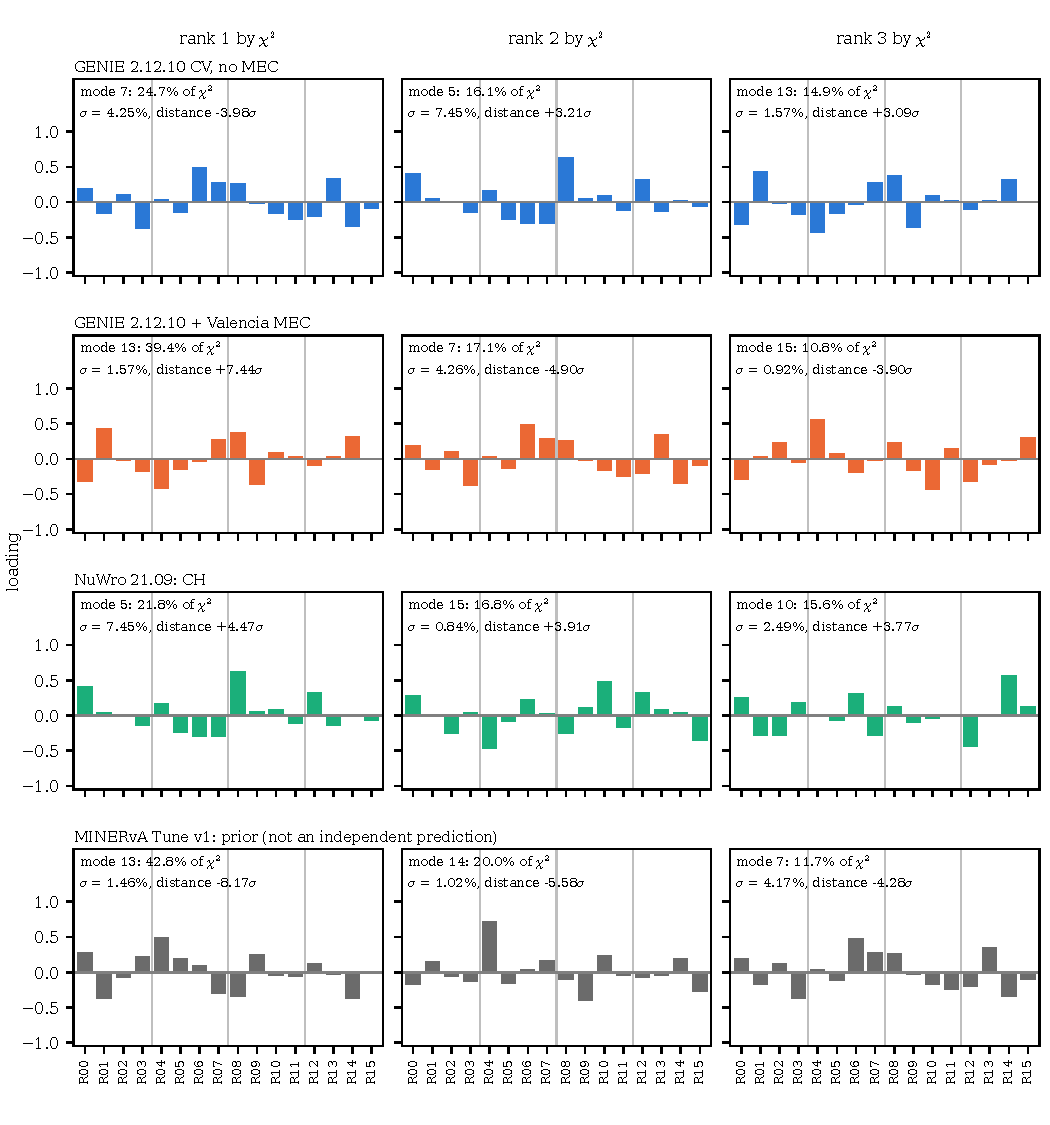
\includegraphics[width=0.85\linewidth]{figures/fd_g_fig_modes.pdf}
  \caption{Several modes contribute to the descriptive distance of each full-grid
  prediction. The panels show the cell loadings for the three largest $\chi^2$
  contributions, using the covariance of fractional residuals from
  $C_{\mathrm{rep}}+V_g$. The distances are descriptive, and the NuWro row uses
  the secondary CH comparison.}
  \label{fig:fived16-modes}
\end{figure}

\subsection{Bias, prior dependence, and numerical stability}
\label{app:bias-prior-stability}

Integrating the 3D result over $E_{\mathrm{avail}}$
leaves a shape difference with the published 2D result. The distance
per bin in the published covariance is 4.98 for the 3D purity marginal
(Fig.~\ref{fig:eavail-marg}) and 4.52 for the refined 3D marginal.

\begin{figure}[tbp]
  \centering
  \includegraphics[width=\textwidth]{eavail_marginal_vs_paper_pull_full}
  \caption{The 3D purity marginal differs from the published 2D result with both signs,
  with the largest positive differences near the high-$p_\parallel$ edge. The
  map and distribution show the muon-plane differences in units of the
  published binwise uncertainties. The comparison is descriptive because the
  results share data.}
  \label{fig:eavail-marg}
\end{figure}

Recovery of injected joint structure varies across cells. The GENIE
sample entering the GiBUU-to-GENIE available-energy ratio used a
mismatched flux (Appendix~\ref{app:choices-after-results}), so the ratio serves as a stress test at
the scale of generator differences. For the three other injected shapes
in Sec.~\ref{sec:higher-dimensional-closure}, the
unfolded shift has the opposite sign in up to \fvval{rec-w-opp-hi} supported
$(E_{\mathrm{avail}},W)$ cells and overshoots in \fvval{rec-w-over-lo} to \fvval{rec-w-over-hi} cells.
In the sixteen-cell bias test, the GiBUU hybrid gives $|z|=\lrval{vr-R02-z-gibuu}$ and
\lrval{vr-R06-z-gibuu} in R02 and R06. For the separate GiBUU available-energy
deformation, the standardized R06 residual rises from $|z|=\fvval{f0b-stage0c_gibuu-zmax}$ to \fvval{f0b-stage0c_gibuu-zmax-nopl}
when the run-period term is removed from the reference covariance.
Figure~\ref{fig:gbdt-bias-spread} compares the size of the bias with
the repeat spread at a fixed iteration count.

\begin{figure}[tbp]
  \centering
  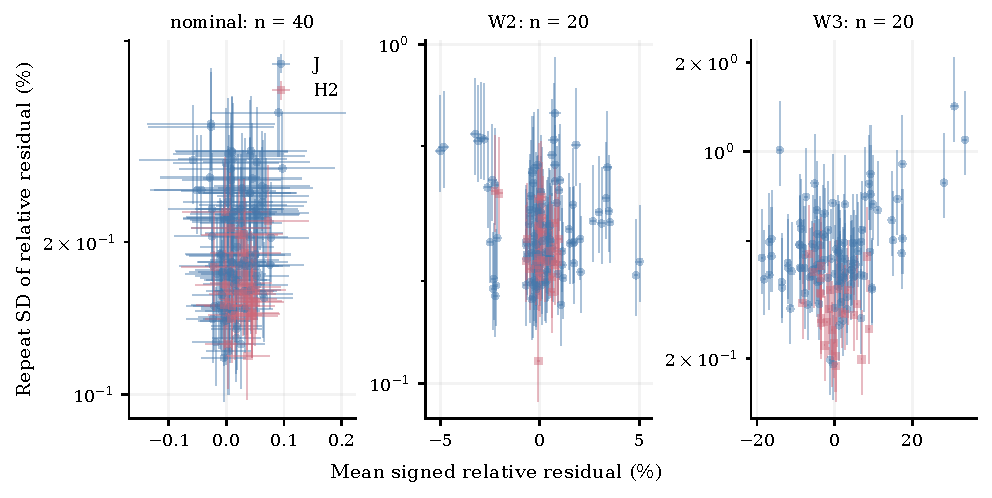
\includegraphics[width=\linewidth]{figures/gbdt_bias_spread.pdf}
  \caption{Bias can exceed the repeat spread for the refined estimator at five
  iterations. The panels show the repeat standard deviation versus the mean
  signed fractional residual at nominal truth and under the GENIE+MEC
  $(E_{\mathrm{avail}},W)$ (W2) and NuWro $(p_T,p_\parallel,E_{\mathrm{avail}})$
  (W3) shape reweightings. Colors distinguish the fine joint (109 cells) and
  coarse joint (27 cells) grids. The ensembles reuse samples from the
  estimator studies.}
  \label{fig:gbdt-bias-spread}
\end{figure}

The prior shifts on data can track the direction of closure bias
without bounding its magnitude (Fig.~\ref{fig:gbdt-prior}).
The largest absolute data shift across the tested priors has medians
of $12.0\%$, $9.6\%$, and $13.4\%$ on the 109 fine joint cells, 27
coarse joint cells, and 39 supported $(E_{\mathrm{avail}},W)$ cells,
respectively. The corresponding 90th percentiles are $38.6\%$,
$22.5\%$, and $39.2\%$. Omitting the GiBUU available-energy
deformation lowers the medians to $11.2\%$, $4.3\%$, and $9.9\%$.
The prespecified median half-width target was $10\%$. The tested envelope
alone exceeds it on the fine joint grid and in the projected plane.
On the coarse joint grid, the median is at least $11.0\%$ under the
study's convention of adding the $1.4\%$ normalization contribution
linearly to the model envelope.

\begin{figure}[H]
  \centering
  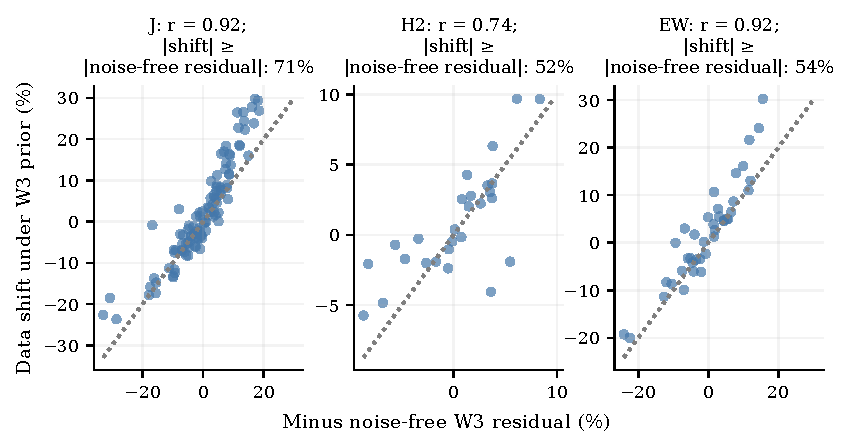
\includegraphics[width=\linewidth]{figures/gbdt_prior_response.pdf}
  \caption{The data shifts under the NuWro $(p_T,p_\parallel,E_{\mathrm{avail}})$ prior
  reweighting (W3) track minus the noise-free closure residual at that truth,
  but the correlation does not bound the bias in any cell. The panels show the
  fine joint, coarse joint, and $(E_{\mathrm{avail}},W)$ grids, each with the
  correlation and the fraction of cells in which the shift is at least as large
  as the residual.}
  \label{fig:gbdt-prior}
\end{figure}

Breaking ties among equal single-precision inputs changes how the tree
learner bins the features. On one pseudo-experiment, perturbations that
preserve ties remove the rounding-induced spread. Perturbing the inputs
to the background-refinement stage alone reproduces the spread. So do
perturbations confined to the OmniFold loop for the 153 test integrals,
with an inconclusive result on the sixteen reporting cells. The tie and
stage tests were separate, so they do not locate the effect in a single
stage.

The paired bootstrap diagnostic supports counting the rounding variance
within the refitted statistical block. For 50 bootstrap replicas with
perturbed counterparts, the paired-to-base spread ratio has median
1.02 and the estimated numerical share of the bootstrap variance
is 0.37. The bootstrap variance is at least as large as the paired
rounding estimate in every supported cell, satisfying the containment
rule of Appendix~\ref{app:multidimensional-statistics}.

\subsection{Alternative algorithms and classifier controls}
\label{app:algorithm-classifier-controls}

The largest differences between \lrval{rg1-K}-iteration binned IBU and the
sixteen-cell result on data are $\fvval{ibu16-dof-R11}\%$ in R11, $\fvval{ibu16-dof-R06}\%$ in R06,
and $\fvval{ibu16-dof-R05}\%$ in R05, expressed relative to the OmniFold integrals.
The R06 difference is \fvval{ibu16-dsig-R06} times its reported standard deviation.
The paired test in Sec.~\ref{sec:higher-dimensional-prior}
establishes sensitivity to the unfolding procedure, including the
response grid used by IBU.

A noise-free comparison with exact binned iteration helps locate the
source of closure residuals. Of 376 cell--deformation pairs with
residuals above $2\%$, 144 have a diagnosis stable under changes in
truth binning and response weighting. The tree approximation dominates
in 15 of these 144 cases. The binned response constrains most of the
retained cases weakly, consistent with regularization accounting for
most residuals in this diagnostic. This reading applies to the selected
cases at the simulated detector response~\cite{NoteRecords2026}.

The detector-level tree classifier shows a nearly diagonal reliability
curve, with a Brier score of approximately 0.25 and an area under the
receiver operating characteristic curve of 0.537. Replacing the trees
with a multilayer perceptron in the 3D purity unfolding gives median
absolute projection differences of $1.20\%$ in $p_T$, $1.36\%$ in
$p_\parallel$, and $0.66\%$ in $E_{\mathrm{avail}}$
(Fig.~\ref{fig:calibration}).

\begin{figure}[H]
  \centering
  \includegraphics[width=\textwidth]{nn_vs_gbdt_full}
  \caption{The largest differences between the multilayer perceptron and the
  gradient-boosted trees occur at the sparsely populated edges of the muon
  spectra. The panels show absolute 3D purity-baseline projections and their
  ratios at five iterations. The comparison is descriptive.}
  \label{fig:calibration}
\end{figure}

% PASS2:
% Source literals kept without a matching value macro. C.1: slice counts
% 14 and 16, LightGBM range 2.64--2.75 over ten seeds, and histogram-based
% result 2.70 +/- 0.04. C.2: 0.02, the corner edges 0.8 and 1.8 GeV, the
% W interval [1.4,1.8) GeV, the scan endpoints, four degrees of freedom,
% and the 16- and 8-cell domains. C.3: 4.98 and 4.52, the grid counts
% 109/27/39, the 90th percentile, envelope medians 12.0/9.6/13.4 and
% 11.2/4.3/9.9, percentiles 38.6/22.5/39.2, the 10% target, 11.0% and
% 1.4%, 153 integrals, and the paired-bootstrap values 50, 1.02, and 0.37.
% C.4: 376, 2%, 144, and the classifier scores 0.25 and 0.537.
% Additional literals with no matching value macro in the supplied set:
% C.1 eigenmode share 9.6% and relative eigenvalues 4e-9, 4e-6, 6e-5.
% C.2 data Pearson coefficients 0.82 and 0.74, migration range 0.58--0.61,
% quadrant thresholds 0.05 and 2.50, and the derived carbon weight 12/13.
% C.4 tree-dominated count 15 and classifier projection differences
% 1.20%, 1.36%, and 0.66%. Retained the figure/records values in the draft.
% All active references resolve against new-labels.md or this file. Legacy
% table labels for omitted tables (tab:fived16-quad-x, tab:fived16-sens,
% tab:fived16-gen-target) have no table here. The author cut fig:eavail and
% fig:ascencio. The old tab:fived16-groups label points to the first of
% the two uncertainty tables. Legacy section labels already assigned to
% the body drafts were left there to avoid duplicate definitions.
